\chapter{Referencial Teórico}
\label{cap:referencial}

 
% computação paralela
\section{Processamento Distribuído ? / Computação Paralela ?}


Com o avanço tecnólogico da última década, o volume crescente de dados sendo gerado, coletado e armazenado tornou o processamento dos dados inviável para um único computador. A quantidade de dados atualmente processados cria a necessidade de computação de alto desempenho, cujo foco sejam os dados.  Como resultado, torna-se crucial substituir a computação tradicional por computação distribuída eficiente. 
É um caminho natural para o processamento de dados em larga escala o uso de \textit{clusters} ~\cite{Lin:2010}.

Clusters são conjuntos de máquinas, ligadas em rede, que comunicam-se através do sistema, trabalhando como se fossem uma única máquina de grande porte. 
Dentre algumas características observadas em um \textit{cluster}, é possível destacar: o baixo custo se comparado a supercomputadores; a proximidade geografica dos nós. altas taxas de transferência nas conexões entre as máquinas e o uso de máquinas homogêneas \cite{Toth:2008}.

Apesar dos computadores em um \textit{cluster} não precisarem processar necessariamente a mesma aplicação, a grande vantagem de tal organização é a habilidade de cada nó processar individualmente uma fração da aplicação, resultando em desempenho que pode ser comparado ao de um supercomputador.
Em geral os computadores de \textit{clusters} são de baixo custo, o que permite que um grande número de máquinas seja interligadas, garantindo grande desempenho e melhor custo-benefício que supercomputadores, o que apresenta grande vantagem. Outro ponto importante é que novas máquinas podem ser facilmente incorporadas  ao \textit{cluster}, tornando-o uma solução mais flexível, principalmente por ser formado por maquinas de capacidade de processamento similar.

\textit{Esta linha de pesquisa envolve vários outros conceitos relacionados à infraestrutura, como comunicação entre os nós, balanceamento de carga e outros discutidos nas próximas seções.}


\subsection{ Princípios de processamento em cluster? distribuído? de grande volumes de dados? }

O processamento de grandes volumes de dados em \textit{clusters} deve suportar alguns princípios para garantir a escalabilidade e o bom desempenho \cite{Bryant:2011}:



\paragraph{Tratamento de dados intrínsecos}
A coleta e manutenção dos dados deve ser funções do sistema e não tarefa dos usuários.  
O sistema deve recuperar informações atualizadas através de rede e realizar cálculos derivados como tarefas em segundo plano. Os usuários devem ser capazes de usar consultas ricos com base no conteúdo e identidade para acessar os dados. 
Mecanismos de confiabilidade, como replicação e de correção de erros devem ser incorporados como parte do sistema, de modo a garantir integridade e disponibilidade dos dados.

\paragraph{Modelo de programação paralelo de alto nível}
O desenvolvedor da aplicação deve fazer uso de primitivas de programação de alto nível, capazes de expressar formas naturais de paralelismo, que não incluam cofigurações específicas de uma máquina. O trabalho de mapear essas computações para a máquina de forma eficiente deve ficar a cargo do sistema, compilador e runtime.

\paragraph{Acesso interativo} 
Os usuários devem ser capazes de executar programas de forma interativa, com variação dos requisitos de computação e armazenamento O sistema deve responder a consultas e cálculos simples rapidamente, e responder aos complexos sem degradar o desempenho geral. Para suportar a computação interativa, deve haver oferta de recursos. O custo consequente do aumento dos recursos ofertados pode ser justificado com base no aumento da produtividade dos usuários do sistema.


\paragraph{Mecanismos escaláveis para garantir alta confiabilidade e disponibilidade}
Um sistema para computação de grandes volumes de dados deve implementar mecanismos de confiabilidade, no qual os dados originais e intermediários são armazenados de forma redundante. Isso permite que no caso de falhas de componente ou dados seja possível refazer a computação. Além disso, a máquina deve identificar e desativar automaticamente componentes que falharam, de modo a não prejudicar o desempenho do sistema e se manter sempre disponível. 


Grandes empresas de serviços de Internet - como Google, Yahoo, Facebook e Amazon - buscam soluções para processamento de dados em grandes conjuntos de máquinas que atendam as características descritas. Com um software que provê tais características é possível alcançar alto grau de escalabilidade e custo-desempenho. 

Dentre as principais propostas está o modelo MapReduce e sua implementação Hadoop, que são soluções escaláveis, capazes de processar grandes volumes de dados, com alto nível de abstração para distribuir a aplicação e mecanismos de tolerância a falhas.

A próxima seção apresenta com mais detalhes o modelo e suas características.

%
%
%\textit{modelos de computação paralela (memória compartilhada, distribuida, threads, paralelismo de dados e map reduce)}
%
% More precise simulations or the simulations of larger problems need greater and greater computing power and memory space. In the last decades, high-performance research included new developments in parallel hard- ware and software technologies, and a steady progress in parallel high-performance computing can be observed.
% Multicore architectures in the form of single multicore processors, shared mem- ory systems of several multicore processors, or clusters of multicore processors with a hierarchical interconnection network will have a large impact on software development.
%
%Parallel programming models provide methods to support the parallel programming.
%
%parallel programming techniques that are neces- sary for developing efficient programs for multicore processors as well as for par- allel cluster systems
%
%
%The goal of a programming model is to provide a mechanism with which the programmer can specify parallel programs. To do so, a set of basic tasks must be supported. A parallel program specifies computations which can be executed in par- allel.
%
%The programming model is at the next higher level of abstraction and describes a parallel computing system in terms of the semantics of the programming lan- guage or programming environment. A parallel programming model specifies the programmer’s view on parallel computer by defining how the programmer can code an algorithm. This view is influenced by the architectural design and the language, compiler, or the runtime libraries and, thus, there exist many different parallel pro- gramming models even for the same architecture. There are several criteria by which the parallel programming models can differ:
%• the level of parallelism which is exploited in the parallel execution (instruction level, statement level, procedural level, or parallel loops);
%• theimplicitoruser-definedexplicitspecificationofparallelism;
%• thewayhowparallelprogrampartsarespecified;
%• the execution mode of parallel units (SIMD or SPMD, synchronous or asyn-
%chronous);
%• themodesandpatternofcommunicationamongcomputingunitsfortheexchange
%of information (explicit communication or shared variables);
%• synchronizationmechanismstoorganizecomputationandcommunicationbetween
%parallel units.
%
%For the software developer, the new hardware development toward multicore architectures is a challenge, since existing software must be restructured toward parallel execution to take advantage of the additional computing resources. In partic- ular, software developers can no longer expect that the increase of computing power can automatically be used by their software products. Instead, additional effort is required at the software level to take advantage of the increased computing power.
%
%There is much research going on in the area of parallel programming languages and environments with the goal of facilitating parallel programming by providing support at the right level of abstraction.


\section{MapReduce}
O MapReduce é um modelo de programação paralela criado pela Google para processamento de grandes volumes de dados em \textit{clusters}. Esse modelo propõe simplificar a computação paralela e ser de fácil uso, abstraindo conceitos complexos da paralelização - como tolerância a falhas, distribuição de dados e balanço de carga - e utilizando duas funções principais: Map e reduce. A complexidade do algoritmo paralelo não é vista pelo desenvolvedor, que pode se ocupar em desenvolver a solução proposta \cite{Dean:2008}.

Esse modelo de programação é inspirado em linguagens funcionais, tendo como base as primitivas Map e reduce.
Os dados de entrada são específicos para cada aplicação, e descritos pelo usuário. A saída é um conjunto de pares no formato (chave, valor).
A função Map é aplicada aos dados de entrada e produz uma lista intermediária de pares (chave, valor). Todos os valores intermediários associados a uma mesma chave são agrupados e enviados à função reduce.
A função reduce é então aplicada para todos os pares intermediários com a mesma chave. A função combina esses valores para formar um conjunto menor de resultados.
Tipicamente, há apenas zero ou um valores de saída em cada função reduce.

O pseudocódigo a seguir apresenta um exemplo de uso do MapReduce, cujo objetivo é contar a quantidade de ocorrências de cada palavra em um documento. A função Map recebe como valor uma linha do documento texto, e como chave o número da linha. Para cada palavra encontrada na linha recebida, a função emite a palavra e a contagem de uma ocorrência. A função Reduce, recebe como chave uma palavra, e uma lista dos valores emitidos pela função Map, associados com a palavra questão. As ocorrências da palavra são agrupadas e a função retorna palavra e seu total de ocorrências.

\begin{lstlisting}[label=some-code,caption=Pseudocódigo do exemplo de contagem de palavras com o MapReduce]
Function Map (Integer chave, String valor):
#chave: numero da linha no arquivo.
#valor: texto da linha correspondente.
listaDePalavras = split (valor)
for palavra in listaDePalavras:
emit (palavra, 1)
Function reduce (String chave, Iterator valores):
#chave: palavra emitida pela funcao Map.
#valores: conjunto de valores emitidos para a chave.
total = 0
for v in valores:
total = total + 1
emit (palavra, total)
\end{lstlisting}

A Figura \ref{fig:Mapreduceexemplo} ilustra o fluxo de execução para este exemplo. A entrada é um arquivo contendo as linhas "Exemplo conta palavras" e "Hadoop exemplo palavras".

\begin{figure}[htb]
\centering
%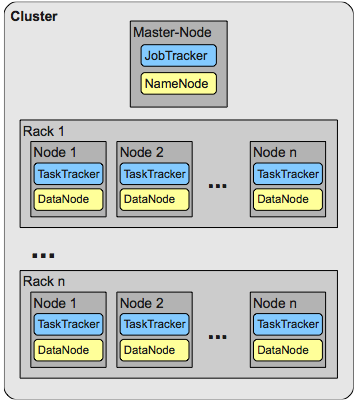
\includegraphics[scale=.65]{figuras/HadoopCluster.png}
\caption{Fluxo simplificado da contagem de palavras com o MapReduce}
\label{fig:Mapreduceexemplo}
\end{figure}

\subsubsection{Arquitetura do MapReduce}
O MapReduce é constituído de uma arquitetura com dois tipos principais de nós: \textit{Master} e \textit{Worker}. O nó mestre tem como função atender requisições de execução dos usuários, gerenciá-las, criar tarefas e distribuí-las entre os nós trabalhadores, que executam as tarefas com base nas funções Map e Reduce definidas pelo usuário.
%Como é possível perceber, trata-se de uma típica arquitetura mestre-escravo (do inglês master-slave) (DUBREUIL; GAGNÉ; PARIZEAU, 2006).
A arquitetura também é inclui um sistema de arquivos distribuídos, onde ficam armazenados os dados de entrada e intermediários.
%Para evitar a transferência excessiva de dados, os \textit{workers} do MapReduce são também nós do sistema de arquivos.


% }

\subsubsection{Visão geral do fluxo de execução}


As chamadas da função map são distribuídas automaticamente entre as diversas máquinas através do particionamento dos dados de entrada em \textit{M} conjuntos. Cada conjunto pode ser processado em paralelo por diferentes máquinas. As chamadas da função reduce são distribuídas pelo do particionamento do conjunto intermediário de pares em \textit{R} partes. O número de partições \textit{R} pode ser definido pelo usuário.

A Figura \ref{fig:mapreduceoverview} ilustra uma o fluxo de uma execução do modelo MapReduce \cite{Dean:2008}. A sequência de ações descrita a seguir explica o que ocorre em cada um dos passos. A numeração dos itens a seguir corresponde à numeração da figura.



 \begin{figure}[htb]
 \centering
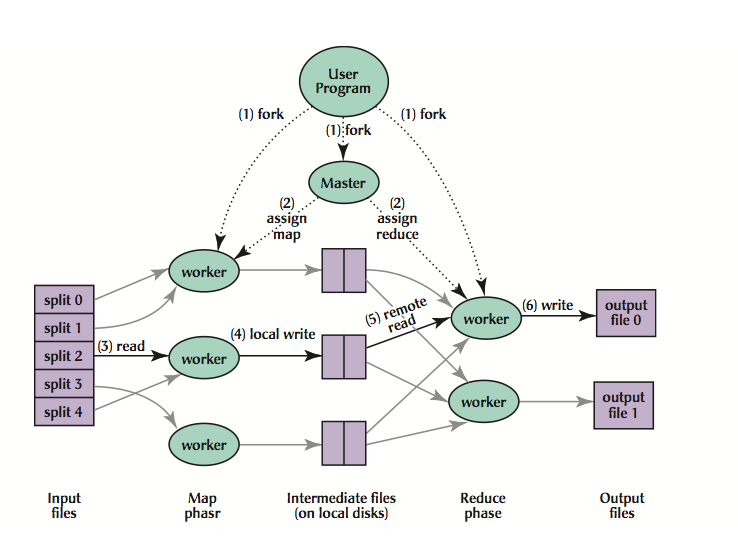
\includegraphics[scale=.65]{figuras/MapReduceOverview.png}
\caption{Visão geral do funcionamento do modelo MapReduce.}
\label{fig:mapreduceoverview}
\end{figure}



\begin{enumerate}
\item A biblioteca MapReduce no programa do usuário primeiro divide os arquivos de entrada em M pedaços. Em seguida, iniciam-se muitas cópias do programa em um cluster de máquinas.

\item Uma das cópias do programa é especial: o mestre (\textit{master}). Os demais são trabalhadores (escravos, slaves) cujo trabalho é atribuído pelo mestre. Existem M tarefas Map e R tarefas Reduce a serem atribuídas. O mestre atribui aos trabalhadores ociosos uma tarefa Map ou uma tarefa Reduce.

\item Um trabalhador que recebe uma tarefa Map lê o conteúdo do fragmento de entrada correspondente. Ele analisa pares (chave, valor), a partir dos dados de entrada e encaminha cada par para a função Map definida pelo usuário. Os pares (chave, valor) intermediários, produzidos pela função Map, são colocados no buffer de memória;

\item Um trabalhador que recebe uma tarefa Map lê o conteúdo do fragmento de entrada correspondente. Ele analisa pares (chave, valor), a partir dos dados de entrada e encaminha cada par para a função Map definida pelo usuário. Os pares (chave, valor) intermediários, produzidos pela função Map, são colocados no buffer de memória;

\item Periodicamente, os pares colocados no buffer são gravados no disco local, divididos em regiões R pela função de particionamento. As localizações desses pares bufferizados no disco local são passadas de volta para o mestre, que é responsável pelo encaminhamento desses locais aos trabalhadores Reduce;

\item Quando um trabalhador Reduce é notificado pelo mestre sobre essas localizações, ele usa chamadas de procedimento remoto para ler os dados no buffer, a partir dos discos locais dos trabalhadores Map. Quando um trabalhador Reduce tiver lido todos os dados intermediários para sua partição, ela é ordenada pela chave intermediária para que todas as ocorrências da mesma chave sejam agrupadas. Se a quantidade de dados intermediários é muito grande para caber na memória, um tipo de ordenação externa é usado;

\item O trabalhador Reduce itera sobre os dados intermediários ordenados e, para cada chave intermediária única encontrada, passa a chave e o conjunto correspondente de valores intermediários para função Reduce do usuário. A saída da função Reduce é anexada a um arquivo de saída final para essa partição Reduce;

\item Quando todas as tarefas Map e Reduce são concluídas, o mestre acorda o programa do usuário. Neste ponto, a chamada MapReduce no programa do usuário retorna para o código do usuário.
              	        	
\end{enumerate}


\subsection{Hadoop}
Uma das implementações mais conhecidas do MapReduce é o Hadoop, desenvolvido por Doug Cutting em 2005 e mantido pela Apache Software Foundation. O Hadoop é uma implementação código aberto em Java do modelo criado pela Google, que provê o gerenciamento de computação distribuída, de maneira escalável e confiável \cite{Hadoop:2010}.

Facebook, Yahoo! e eBay utilizam o ambiente Hadoop em seus \textit{clusters} para processar diariamente terabytes de dados e logs de eventos para detecção de spam, \textit{business intelligence} e diferentes tipos de otimização \cite{Cherkasova:2011}.

%Os conceitos de nó \textit{Master} e \textit{Worker} do MapReduce, são respectivamente denominados JobTracker e TaskTracker no Hadoop. O sistema de arquivos também foi incorpo

O modelo MapReduce foi criado para permitir o processamento em conjuntos de centenas de máquinas de maneira transparente, o que significa que o usuário não deve ser preocupar com mecanismos de tolerância a falhas, que deve ser provido pelo sistema \cite{Dean:2008}. 
Um dos principais benefícios do Hadoop é a sua capacidade de lidar com falhas, sejam de disco, processos, ou de nós, e permitir que o trabalho do usuário possa ser concluído.

O sistema é capaz de verificar e substituir nós quando ocorre alguma falha. O nó mestre envia mensagens periódicas aos demais nós para verificar seu estado. Se nenhuma resposta é recebida, o mestre identifica que houve uma falha neste nó. 
As tarefas que não foram executadas são reescalonadas para os demais nós. O mecanismo de replicação garante que sempre haja um número determinado de cópias dos dados, e caso um dos nós de armazenamento seja perdido, os demais se encarregam de realizar uma nova replicação \cite{Hadoop:2010}.



\subsubsection{HDFS}


O \textit{ Hadoop Distributed File System} (HDFS) é um sistema de arquivos distribuído desenvolvido para armazenar grandes conjuntos de dados e ser altamente tolerante a falhas \cite{Hadoop:2010}.
A plataforma Hadoop suporta diversos sistemas de arquivos distintos, como Amazon S3 (Native e Block-based), CloudStore, HAR, sistemas mantidos por servidores FTP e HTTP, Local (destinado a unidades de armazenamento conectadas localmente), mas fornece o HDSF como sistema de arquivos padrão.

A arquitetura do HDFS também é do tipo mestre-escravos.
O nó mestre (\textit{NameNode}) é responsável por manter e controlar todos os metadados do sistema de arquivos e gerenciar a localização dos dados. Também é responsável por outras atividades, como por exemplo, balanceamento de carga, \textit{garbage collection}, e atendimento a requisições dos clientes.
Os nós escravos (\textit{DataNode}) são responsáveis por armazenar e transmitir os dados aos usuários que os requisitarem.

A Figura \ref{fig:hdfs} ilustra a arquitetura do sistema de arquivos distribuídos.
O Namenode gerencia e manipula todas as informações dos arquivos, tal como a localização e o acesso. Os Datanodes se encarregam da leitura e escrita das informações nos sistemas de arquivos cliente.

\begin{figure}[htb]
\centering
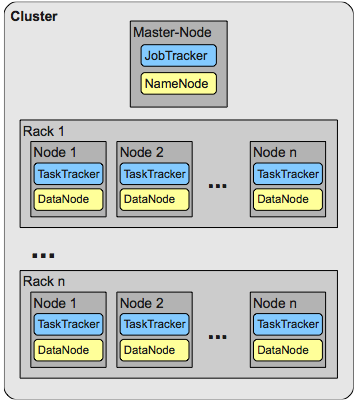
\includegraphics[scale=.65]{figuras/HadoopCluster.png}
\caption{Visão abstrata do cluster.}
\label{fig:hdfs}
\end{figure}

O HDFS incorpora funcionalidades que têm grande impacto no desempenho geral do sistema.
Uma delas é conhecida como \textit{rack awareness}. Com esse recurso, o sistema de arquivos é capaz de identificar os DataNodes que pertencem a um mesmo \textit{rack}, e distribuir as réplicas de maneira mais inteligente, aumentando a performance e confiabilidade do sistema.
A outra é a distribuição dos dados. O sistema de arquivos busca manter um balanceamento na ocupação das unidades de armazenamento, e o \textit{framework}, busca atribuir tarefas a um \textit{worker} que possua, em sua unidade de armazenamento local os dados que devem ser processados.
Assim, quando executa-se grandes operações MapReduce com um número significante de nós, a maioria dos dados são lidos localmente e o consumo de banda é mínimo.





\section{Ordenação}


%
%Um grande número de aplicações paralelas possui uma fase de computação intensa, na qual uma lista de elementos deve ser ordenada com base em algum de seus atributos. Um exemplo é o algoritmo de Page Rank \cite{Page:1999} da Google: as páginas de resultado de uma consulta são classificadas de acordo com sua relevância, e então precisam ser ordenadas de maneira eficiente \cite{Kale:2010}.
%No exemplo do Page Rank, o número de páginas a serem ordenadas é enorme, e elas são recolhidas de diversos servidores da Google; é uma questão fundamental escolher algoritmo paralelo com o melhor desempenho dentre as soluções possíveis.
%
%Na criação de algoritmos de ordenação paralela, é ponto fundamental ordenar coletivamente os dados de cada processo individual, de forma a utilizar todas as unidades de processamento e minimizar os custos de redistribuição de chaves entre os processadores.
%\label{cap:ordenacao}
%
%\begin{itemize}
%\item importância da ordenação paralela
%\item formas de ordenação: memória e disco
%\item grandes dados: apenas disco
%\item grandes dados: problematização (tempo, limite de memória)
%\item grandes dados: sort benchmark
%\end{itemize}
%
%
%\begin{itemize}
%\item algoritmos de ordenação paralelos
%\item funcionamento geral
%\item condições / ingredientes / limites
%\item diferentes algoritmos para diferentes aplicações
%\item descrição de algoritmos (e diagramas): sample sort, quick sort
%
%\end{itemize}



A ordenação em memória interna é caracterizada pelo armazenamento de todos os registros na memória principal, onde seus acessos são feitos diretamente pelo processador. Essa ordenação é possível apenas quando a quantidade de dados é pequena o suficiente para ser armazenada em memória. 

Quando a ordenação é feita em um grande conjunto de dados, que não podem ser armazenados em memória principal a ordenação é chamada externa. Apesar do problema nos dois casos ser o mesmo (rearranjar os registros de um arquivo em ordem ascendente ou descendente), não é possível usar as mesmas estratégias da ordenação interna, pois o acesso aos dados é feito em discos, cujo tempo de acesso é muito superior ao da memória principal.  %[Ziviani 2007, Knuth 1973].

Na ordenação externa, os itens que não estão na memória principal devem ser buscados em memória secundária e trazidos para a memória principal, para assim serem comparados. Esse processo se repete inúmeras vezes, o que o torna lento, uma vez que os processadores ficam grande parte do tempo ociosos à espera da chegada dos dados à memória principal para serem processados. Por esse motivo, a grande ênfase de um método de ordenação externa deve ser na minimização do número de vezes que cada item é transferido entre a memória interna e a memória externa. Além disso, cada transferência deve ser realizada de forma tão eficiente quanto as características dos equipamentos disponíveis permitam [Ziviani 2007].



\section{Algoritmos de Ordenação Paralela}

\subsubsection*{Condições de implementação de algoritmos paralelos de ordenação}

\paragraph*{  Habilidade de explorar distribuições iniciais parcialmente ordenadas}
Alguns algoritmos podem se beneficiar de cenários nos quais a sequência de entrada dos dados é mesma, ou pouco alterada. Nesse caso, é possível obter melhor desempenho ao realizar menos trabalho e movimentação de dados.
Se a alteração na posição dos elementos da sequência é pequena o suficiente, grande parte dos processadores mantém seus dados iniciais e precisa se comunicar apenas com os processadores vizinhos.


\paragraph*{Movimentação dos dados}
A movimentação de dados entre processadores deve ser mínima durante a execução do algoritmo. Em um sistema de memória distribuída, a quantidade de dados a ser movimentada é um ponto crítico, pois o custo de troca de dados pode dominar o custo de execução total e limitar a escalabilidade.


\paragraph*{Balanceamento de carga}
O algoritmo de ordenação paralela deve assegurar o balanceamento de carga ao distribuir os dados entre os processadores. Cada processador deve receber uma parcela equilibrada dos dados para ordenar, uma vez que o tempo de execução da aplicação é tipicamente limitada pela execução do processador mais sobrecarregado.

\paragraph*{Latência de comunicação}
A latência de comunicação é definida como o tempo médio necessário para enviar uma mensagem de um processador a outro.
Em grandes sistemas distribuídos, reduzir o tempo de latência se torna muito importante.

\paragraph*{Sobreposição de comunicação e computação}
Em qualquer aplicação paralela, existem tarefas com focos em computação e comunicação. A sobreposição de tais tarefas permite que sejam feitas tarefas de processamento e ao mesmo tempo operações de entrada e saída de dados, evitando que os recursos fiquem ociosos durante o intervalo de tempo necessário para a transmissão da carga de trabalho.

\subsection{Sample Sort}
%O algoritmo de Ordenação por Amostragem [White 2009, Venner 2009] é um método de ordenação externa para ordenar grandes quantidades de dados. A ideia desse algoritmo é dividir um conjunto de dados a ser ordenado em subconjuntos (partições) de forma que os elementos da partição à esquerda sejam menores do que os elementos à direita da partição, isto é, todas as chaves da partição i são menores que as chaves da partição i + 1. Cada uma das partições é designada a um processador para ordenação (ordenação interna) e, assim, é produzido um conjunto de arquivos ordenados que, se concatenados, formam um arquivo globalmente ordenado.
%
%A divisão dos dados em partições (particionamento) é feita por meio de uma estratégia de amostragem. Essa estratégia baseia-se na análise de um subconjunto de dados, denomi- nado amostra, ao invés de todo o conjunto, para estimar a distribuição de chaves e, assim, construir partições balanceadas.
%
%Existem três tipos de estratégias de amostragem: SplitSampler, IntervalSampler e Ran- domSampler. O SplitSampler seleciona apenas os n primeiros registros do arquivo para for- mar a amostra. Já o IntervalSampler forma a amostra por meio da escolha de chaves em intervalos regulares no arquivo. No RandomSampler, a amostra é constituída por chaves selecionadas aleatoriamente no conjunto.
%
%Após a formação das amostras, são definidos os limites para as partições, isto é, o intervalo de valores compreendido por cada partição. A quantidade de limites amostrados (qla) é determinada pelo equação: qla = np - 1, onde np é o número de partições (np = nc x nmaq, sendo nc o número de cores e nmaq o número de máquinas). As informações das partições são armazenadas em um arquivo e transmitidas para as máquinas participantes por meio de cache distribuído.
%
%O melhor tipo de estratégia de amostragem é determinado pela entrada de dados. Para arquivos quase ordenados, o SplitSampler não é recomendado, uma vez que não seleciona as chaves de todo o conjunto e, assim, não produz bons resultados. Nesse caso, a melhor escolha é o IntervalSampler pelo fato de selecionar chaves que representam melhor a distribuição do conjunto. O RandomSampler é considerado um bom amostrador de propósito geral [White 2009], por isso será utilizado neste trabalho.
%
%O RandomSampler apresenta os seguintes parâmetros de balanceamento: probabilidade de escolha de uma chave, o número máximo de amostras a serem selecionadas para realizar a amostragem e o número máximo de partições que podem ser utilizadas. Ele termina quando algum dos parâmetros é atingido.
%
%A Figura 4.6 apresenta um esquema da estrutura de funcionamento do algoritmo, quando implementado em MapReduce no ambiente Hadoop. O algoritmo pode ser di- vidido em duas fases: Map e Reduce.
%
%Na fase Map, os arquivos de entrada são lidos, ocorre a formação do vetor inicial e dos pares (chave, valor) dos valores lidos (passos 1.1 e 1.2). Depois disso, os dados são divididos em partições cujo número é determinado pelo número de máquinas e seus núcleos de processamento (passo 1.3). No exemplo apresentado, são utilizados dois núcleos de pro- cessamento (cores). Portanto, existem duas partições e, dessa forma, deve ser escolhido apenas um limite para as partições. Esse limite é definido por meio da seleção do ele- mento que melhor representa a distribuição de chaves na amostra formada pela estratégia RandomSampler. Para esse exemplo o limite escolhido foi o número 13, o que implica que em uma partição estarão valores menores e iguais a 13 e, na outra, valores maiores que 13. Por meio de cache distribuído, as informações das partições são transmitidas para as máquinas participantes e os dados particionados. Cada partição é então atribuída a uma tarefa Reduce (processador) diferente.
%
%Na fase Reduce, os dados são ordenados localmente (passo 2.1), ou seja, em cada processador os dados são ordenados na memória interna. Para essa ordenação, avalia-se a profundidade da árvore de recursão e, se ela for baixa, utiliza-se o algoritmo QuickSort. Caso contrário, o HeapSort é utilizado [White 2009]. Após isso, os dados retornam para a máquina master, onde são concatenados, formando o vetor ordenado.O balanceamento das partições, ou seja, a formação de partições aproximadamente iguais no tamanho é muito importante para o algoritmo de Ordenação por Amostragem, pois evita que os tempos de ordenação sejam dominados por um único processador. Em outras palavras, o equilíbrio das partições reduz a possibilidade de que um processador esteja ocioso, enquanto outro processador está sobrecarregado, situação que comprometeria o desempenho do algoritmo [White 2009].

\subsection{Quick Sort}

 